% Graphic for TeX using PGF
% Title: C:\Users\Nicolas Chicaiza\Sourcetree\Metodología de la Investigación\Enfoque Marco Lógico\Esquemas\Árbol de Participación\arbolParticipacion.dia
% Creator: Dia v0.97.2
% CreationDate: Mon May 03 01:11:19 2021
% For: Nicolas Chicaiza
% \usepackage{tikz}
% The following commands are not supported in PSTricks at present
% We define them conditionally, so when they are implemented,
% this pgf file will use them.
\ifx\du\undefined
  \newlength{\du}
\fi
\setlength{\du}{15\unitlength}
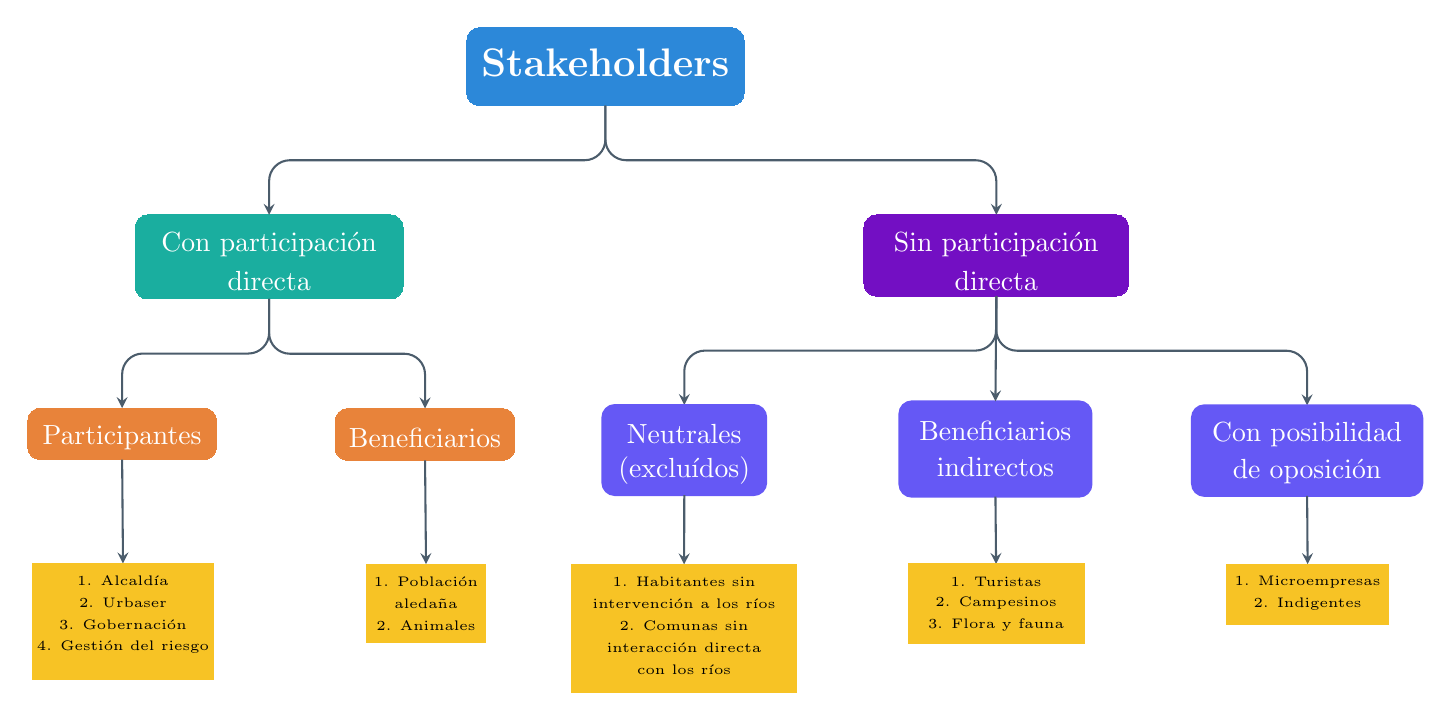
\begin{tikzpicture}[scale = 2.5]
    \pgftransformxscale{1.000000}
    \pgftransformyscale{-1.000000}
    \definecolor{dialinecolor}{rgb}{0.000000, 0.000000, 0.000000}
    \pgfsetstrokecolor{dialinecolor}
    \definecolor{dialinecolor}{rgb}{1.000000, 1.000000, 1.000000}
    \pgfsetfillcolor{dialinecolor}
    \pgfsetlinewidth{0.000000\du}
    \pgfsetdash{}{0pt}
    \pgfsetdash{}{0pt}
    \pgfsetroundjoin
    {\pgfsetcornersarced{\pgfpoint{0.300000\du}{0.300000\du}}\definecolor{dialinecolor}{rgb}{0.172549, 0.533333, 0.850980}
    \pgfsetfillcolor{dialinecolor}
    \fill (49.907800\du,8.337130\du)--(49.907800\du,9.087734\du)--(52.579713\du,9.087734\du)--(52.579713\du,8.337130\du)--cycle;
    }{\pgfsetcornersarced{\pgfpoint{0.300000\du}{0.300000\du}}\definecolor{dialinecolor}{rgb}{0.172549, 0.533333, 0.850980}
    \pgfsetstrokecolor{dialinecolor}
    \draw (49.907800\du,8.337130\du)--(49.907800\du,9.087734\du)--(52.579713\du,9.087734\du)--(52.579713\du,8.337130\du)--cycle;
    }% setfont left to latex
    \definecolor{dialinecolor}{rgb}{1.000000, 1.000000, 1.000000}
    \pgfsetstrokecolor{dialinecolor}
    \node at (51.243756\du,8.674630\du){\Large \textbf{\textcolor{white}{Stakeholders}}};
    \pgfsetlinewidth{0.000000\du}
    \pgfsetdash{}{0pt}
    \pgfsetdash{}{0pt}
    \pgfsetroundjoin
    {\pgfsetcornersarced{\pgfpoint{0.300000\du}{0.300000\du}}\definecolor{dialinecolor}{rgb}{0.450980, 0.058824, 0.764706}
    \pgfsetfillcolor{dialinecolor}
    \fill (53.735000\du,10.140888\du)--(53.735000\du,10.923562\du)--(56.285803\du,10.923562\du)--(56.285803\du,10.140888\du)--cycle;
    }{\pgfsetcornersarced{\pgfpoint{0.300000\du}{0.300000\du}}\definecolor{dialinecolor}{rgb}{0.450980, 0.058824, 0.764706}
    \pgfsetstrokecolor{dialinecolor}
    \draw (53.735000\du,10.140888\du)--(53.735000\du,10.923562\du)--(56.285803\du,10.923562\du)--(56.285803\du,10.140888\du)--cycle;
    }\pgfsetlinewidth{0.050000\du}
    \pgfsetdash{}{0pt}
    \pgfsetdash{}{0pt}
    \pgfsetroundjoin
    \pgfsetbuttcap
    {
    \definecolor{dialinecolor}{rgb}{0.294118, 0.360784, 0.419608}
    \pgfsetfillcolor{dialinecolor}
    % was here!!!
    \pgfsetarrowsend{stealth}
    {\pgfsetcornersarced{\pgfpoint{0.500000\du}{0.500000\du}}\definecolor{dialinecolor}{rgb}{0.294118, 0.360784, 0.419608}
    \pgfsetstrokecolor{dialinecolor}
    \draw (51.243756\du,9.087734\du)--(51.243756\du,9.614311\du)--(55.010402\du,9.614311\du)--(55.010402\du,10.140888\du);
    }}
    % setfont left to latex
    \definecolor{dialinecolor}{rgb}{1.000000, 1.000000, 1.000000}
    \pgfsetstrokecolor{dialinecolor}
    \node at (55.010402\du,10.423388\du){\textcolor{white}{Sin participación}};
    % setfont left to latex
    \definecolor{dialinecolor}{rgb}{1.000000, 1.000000, 1.000000}
    \pgfsetstrokecolor{dialinecolor}
    \node at (55.010402\du,10.776165\du){\textcolor{white}{directa}};
    \pgfsetlinewidth{0.000000\du}
    \pgfsetdash{}{0pt}
    \pgfsetdash{}{0pt}
    \pgfsetroundjoin
    {\pgfsetcornersarced{\pgfpoint{0.300000\du}{0.300000\du}}\definecolor{dialinecolor}{rgb}{0.101961, 0.682353, 0.623529}
    \pgfsetfillcolor{dialinecolor}
    \fill (46.713200\du,10.140888\du)--(46.713200\du,10.951084\du)--(49.293356\du,10.951084\du)--(49.293356\du,10.140888\du)--cycle;
    }{\pgfsetcornersarced{\pgfpoint{0.300000\du}{0.300000\du}}\definecolor{dialinecolor}{rgb}{0.101961, 0.682353, 0.623529}
    \pgfsetstrokecolor{dialinecolor}
    \draw (46.713200\du,10.140888\du)--(46.713200\du,10.951084\du)--(49.293356\du,10.951084\du)--(49.293356\du,10.140888\du)--cycle;
    }% setfont left to latex
    \definecolor{dialinecolor}{rgb}{1.000000, 1.000000, 1.000000}
    \pgfsetstrokecolor{dialinecolor}
    \node at (48.003278\du,10.423388\du){\textcolor{white}{Con participación}};
    % setfont left to latex
    \definecolor{dialinecolor}{rgb}{1.000000, 1.000000, 1.000000}
    \pgfsetstrokecolor{dialinecolor}
    \node at (48.003278\du,10.776165\du){\textcolor{white}{directa}};
    \pgfsetlinewidth{0.050000\du}
    \pgfsetdash{}{0pt}
    \pgfsetdash{}{0pt}
    \pgfsetroundjoin
    \pgfsetbuttcap
    {
    \definecolor{dialinecolor}{rgb}{0.294118, 0.360784, 0.419608}
    \pgfsetfillcolor{dialinecolor}
    % was here!!!
    \pgfsetarrowsend{stealth}
    {\pgfsetcornersarced{\pgfpoint{0.500000\du}{0.500000\du}}\definecolor{dialinecolor}{rgb}{0.294118, 0.360784, 0.419608}
    \pgfsetstrokecolor{dialinecolor}
    \draw (51.243756\du,9.087734\du)--(51.243756\du,9.614311\du)--(48.003278\du,9.614311\du)--(48.003278\du,10.140888\du);
    }}
    \pgfsetlinewidth{0.050000\du}
    \pgfsetdash{}{0pt}
    \pgfsetdash{}{0pt}
    \pgfsetroundjoin
    \pgfsetbuttcap
    {
    \definecolor{dialinecolor}{rgb}{0.294118, 0.360784, 0.419608}
    \pgfsetfillcolor{dialinecolor}
    % was here!!!
    \pgfsetarrowsend{stealth}
    {\pgfsetcornersarced{\pgfpoint{0.500000\du}{0.500000\du}}\definecolor{dialinecolor}{rgb}{0.294118, 0.360784, 0.419608}
    \pgfsetstrokecolor{dialinecolor}
    \draw (48.003278\du,10.951084\du)--(48.003278\du,11.478886\du)--(49.505825\du,11.478886\du)--(49.505825\du,12.006688\du);
    }}
    \pgfsetlinewidth{0.050000\du}
    \pgfsetdash{}{0pt}
    \pgfsetdash{}{0pt}
    \pgfsetroundjoin
    \pgfsetbuttcap
    {
    \definecolor{dialinecolor}{rgb}{0.294118, 0.360784, 0.419608}
    \pgfsetfillcolor{dialinecolor}
    % was here!!!
    \pgfsetarrowsend{stealth}
    {\pgfsetcornersarced{\pgfpoint{0.500000\du}{0.500000\du}}\definecolor{dialinecolor}{rgb}{0.294118, 0.360784, 0.419608}
    \pgfsetstrokecolor{dialinecolor}
    \draw (48.003278\du,10.951084\du)--(48.003278\du,11.477036\du)--(46.586887\du,11.477036\du)--(46.586887\du,12.002988\du);
    }}
    \pgfsetlinewidth{0.000000\du}
    \pgfsetdash{}{0pt}
    \pgfsetdash{}{0pt}
    \pgfsetroundjoin
    {\pgfsetcornersarced{\pgfpoint{0.300000\du}{0.300000\du}}\definecolor{dialinecolor}{rgb}{0.909804, 0.513726, 0.227451}
    \pgfsetfillcolor{dialinecolor}
    \fill (45.677300\du,12.002988\du)--(45.677300\du,12.499253\du)--(47.496475\du,12.499253\du)--(47.496475\du,12.002988\du)--cycle;
    }{\pgfsetcornersarced{\pgfpoint{0.300000\du}{0.300000\du}}\definecolor{dialinecolor}{rgb}{0.909804, 0.513726, 0.227451}
    \pgfsetstrokecolor{dialinecolor}
    \draw (45.677300\du,12.002988\du)--(45.677300\du,12.499253\du)--(47.496475\du,12.499253\du)--(47.496475\du,12.002988\du)--cycle;
    }\pgfsetlinewidth{0.000000\du}
    \pgfsetdash{}{0pt}
    \pgfsetdash{}{0pt}
    \pgfsetroundjoin
    {\pgfsetcornersarced{\pgfpoint{0.300000\du}{0.300000\du}}\definecolor{dialinecolor}{rgb}{0.909804, 0.513726, 0.227451}
    \pgfsetfillcolor{dialinecolor}
    \fill (48.639800\du,12.006688\du)--(48.639800\du,12.506686\du)--(50.371850\du,12.506686\du)--(50.371850\du,12.006688\du)--cycle;
    }{\pgfsetcornersarced{\pgfpoint{0.300000\du}{0.300000\du}}\definecolor{dialinecolor}{rgb}{0.909804, 0.513726, 0.227451}
    \pgfsetstrokecolor{dialinecolor}
    \draw (48.639800\du,12.006688\du)--(48.639800\du,12.506686\du)--(50.371850\du,12.506686\du)--(50.371850\du,12.006688\du)--cycle;
    }% setfont left to latex
    \definecolor{dialinecolor}{rgb}{1.000000, 1.000000, 1.000000}
    \pgfsetstrokecolor{dialinecolor}
    \node at (46.586887\du,12.292920\du){\textcolor{white}{Participantes}};
    % setfont left to latex
    \definecolor{dialinecolor}{rgb}{1.000000, 1.000000, 1.000000}
    \pgfsetstrokecolor{dialinecolor}
    \node at (49.505825\du,12.289188\du){\textcolor{white}{Beneficiarios}};
    \pgfsetlinewidth{0.050000\du}
    \pgfsetdash{}{0pt}
    \pgfsetdash{}{0pt}
    \pgfsetroundjoin
    \pgfsetbuttcap
    {
    \definecolor{dialinecolor}{rgb}{0.294118, 0.360784, 0.419608}
    \pgfsetfillcolor{dialinecolor}
    % was here!!!
    \pgfsetarrowsend{stealth}
    {\pgfsetcornersarced{\pgfpoint{0.500000\du}{0.500000\du}}\definecolor{dialinecolor}{rgb}{0.294118, 0.360784, 0.419608}
    \pgfsetstrokecolor{dialinecolor}
    \draw (55.010402\du,10.923562\du)--(55.010402\du,11.449839\du)--(58.005318\du,11.449839\du)--(58.005318\du,11.976115\du);
    }}
    \pgfsetlinewidth{0.050000\du}
    \pgfsetdash{}{0pt}
    \pgfsetdash{}{0pt}
    \pgfsetroundjoin
    \pgfsetbuttcap
    {
    \definecolor{dialinecolor}{rgb}{0.294118, 0.360784, 0.419608}
    \pgfsetfillcolor{dialinecolor}
    % was here!!!
    \pgfsetarrowsend{stealth}
    {\pgfsetcornersarced{\pgfpoint{0.500000\du}{0.500000\du}}\definecolor{dialinecolor}{rgb}{0.294118, 0.360784, 0.419608}
    \pgfsetstrokecolor{dialinecolor}
    \draw (55.010402\du,10.923562\du)--(55.010402\du,11.448589\du)--(52.003848\du,11.448589\du)--(52.003848\du,11.973615\du);
    }}
    \pgfsetlinewidth{0.050000\du}
    \pgfsetdash{}{0pt}
    \pgfsetdash{}{0pt}
    \pgfsetroundjoin
    {\pgfsetcornersarced{\pgfpoint{0.300000\du}{0.300000\du}}\definecolor{dialinecolor}{rgb}{0.396078, 0.345098, 0.960784}
    \pgfsetfillcolor{dialinecolor}
    \fill (51.214800\du,11.973615\du)--(51.214800\du,12.840273\du)--(52.792896\du,12.840273\du)--(52.792896\du,11.973615\du)--cycle;
    }{\pgfsetcornersarced{\pgfpoint{0.300000\du}{0.300000\du}}\definecolor{dialinecolor}{rgb}{0.396078, 0.345098, 0.960784}
    \pgfsetstrokecolor{dialinecolor}
    \draw (51.214800\du,11.973615\du)--(51.214800\du,12.840273\du)--(52.792896\du,12.840273\du)--(52.792896\du,11.973615\du)--cycle;
    }\pgfsetlinewidth{0.050000\du}
    \pgfsetdash{}{0pt}
    \pgfsetdash{}{0pt}
    \pgfsetroundjoin
    {\pgfsetcornersarced{\pgfpoint{0.300000\du}{0.300000\du}}\definecolor{dialinecolor}{rgb}{0.396078, 0.345098, 0.960784}
    \pgfsetfillcolor{dialinecolor}
    \fill (56.896000\du,11.976115\du)--(56.896000\du,12.848581\du)--(59.114637\du,12.848581\du)--(59.114637\du,11.976115\du)--cycle;
    }{\pgfsetcornersarced{\pgfpoint{0.300000\du}{0.300000\du}}\definecolor{dialinecolor}{rgb}{0.396078, 0.345098, 0.960784}
    \pgfsetstrokecolor{dialinecolor}
    \draw (56.896000\du,11.976115\du)--(56.896000\du,12.848581\du)--(59.114637\du,12.848581\du)--(59.114637\du,11.976115\du)--cycle;
    }\pgfsetlinewidth{0.050000\du}
    \pgfsetdash{}{0pt}
    \pgfsetdash{}{0pt}
    \pgfsetroundjoin
    {\pgfsetcornersarced{\pgfpoint{0.300000\du}{0.300000\du}}\definecolor{dialinecolor}{rgb}{0.396078, 0.345098, 0.960784}
    \pgfsetfillcolor{dialinecolor}
    \fill (54.077300\du,11.938288\du)--(54.077300\du,12.856014\du)--(55.926869\du,12.856014\du)--(55.926869\du,11.938288\du)--cycle;
    }{\pgfsetcornersarced{\pgfpoint{0.300000\du}{0.300000\du}}\definecolor{dialinecolor}{rgb}{0.396078, 0.345098, 0.960784}
    \pgfsetstrokecolor{dialinecolor}
    \draw (54.077300\du,11.938288\du)--(54.077300\du,12.856014\du)--(55.926869\du,12.856014\du)--(55.926869\du,11.938288\du)--cycle;
    }\pgfsetlinewidth{0.050000\du}
    \pgfsetdash{}{0pt}
    \pgfsetdash{}{0pt}
    \pgfsetbuttcap
    {
    \definecolor{dialinecolor}{rgb}{0.294118, 0.360784, 0.419608}
    \pgfsetfillcolor{dialinecolor}
    % was here!!!
    \pgfsetarrowsend{stealth}
    \definecolor{dialinecolor}{rgb}{0.294118, 0.360784, 0.419608}
    \pgfsetstrokecolor{dialinecolor}
    \draw (55.010402\du,10.923562\du)--(55.002085\du,11.938288\du);
    }
    % setfont left to latex
    \definecolor{dialinecolor}{rgb}{1.000000, 1.000000, 1.000000}
    \pgfsetstrokecolor{dialinecolor}
    \node at (52.003848\du,12.256115\du){\textcolor{white}{Neutrales}};
    % setfont left to latex
    \definecolor{dialinecolor}{rgb}{1.000000, 1.000000, 1.000000}
    \pgfsetstrokecolor{dialinecolor}
    \node at (52.003848\du,12.608893\du){\textcolor{white}{(excluídos)}};
    % setfont left to latex
    \definecolor{dialinecolor}{rgb}{1.000000, 1.000000, 1.000000}
    \pgfsetstrokecolor{dialinecolor}
    \node at (55.002085\du,12.220788\du){\textcolor{white}{Beneficiarios}};
    % setfont left to latex
    \definecolor{dialinecolor}{rgb}{1.000000, 1.000000, 1.000000}
    \pgfsetstrokecolor{dialinecolor}
    \node at (55.002085\du,12.573565\du){\textcolor{white}{indirectos}};
    % setfont left to latex
    \definecolor{dialinecolor}{rgb}{1.000000, 1.000000, 1.000000}
    \pgfsetstrokecolor{dialinecolor}
    \node at (58.005318\du,12.258615\du){\textcolor{white}{Con posibilidad}};
    % setfont left to latex
    \definecolor{dialinecolor}{rgb}{1.000000, 1.000000, 1.000000}
    \pgfsetstrokecolor{dialinecolor}
    \node at (58.005318\du,12.611393\du){\textcolor{white}{de oposición}};
    \pgfsetlinewidth{0.050000\du}
    \pgfsetdash{}{0pt}
    \pgfsetdash{}{0pt}
    \pgfsetbuttcap
    {
    \definecolor{dialinecolor}{rgb}{0.294118, 0.360784, 0.419608}
    \pgfsetfillcolor{dialinecolor}
    % was here!!!
    \pgfsetarrowsend{stealth}
    \definecolor{dialinecolor}{rgb}{0.294118, 0.360784, 0.419608}
    \pgfsetstrokecolor{dialinecolor}
    \draw (46.586887\du,12.499253\du)--(46.595303\du,13.500100\du);
    }
    \pgfsetlinewidth{0.000000\du}
    \pgfsetdash{}{0pt}
    \pgfsetdash{}{0pt}
    \pgfsetmiterjoin
    \definecolor{dialinecolor}{rgb}{0.968627, 0.764706, 0.145098}
    \pgfsetfillcolor{dialinecolor}
    \fill (45.727300\du,13.500100\du)--(45.727300\du,14.616879\du)--(47.463306\du,14.616879\du)--(47.463306\du,13.500100\du)--cycle;
    \definecolor{dialinecolor}{rgb}{0.968627, 0.764706, 0.145098}
    \pgfsetstrokecolor{dialinecolor}
    \draw (45.727300\du,13.500100\du)--(45.727300\du,14.616879\du)--(47.463306\du,14.616879\du)--(47.463306\du,13.500100\du)--cycle;
    % setfont left to latex
    \definecolor{dialinecolor}{rgb}{0.176471, 0.231373, 0.270588}
    \pgfsetstrokecolor{dialinecolor}
    \node at (46.595303\du,13.670100\du){\tiny 1. Alcaldía};
    % setfont left to latex
    \definecolor{dialinecolor}{rgb}{0.176471, 0.231373, 0.270588}
    \pgfsetstrokecolor{dialinecolor}
    \node at (46.595303\du,13.881767\du){\tiny 2. Urbaser};
    % setfont left to latex
    \definecolor{dialinecolor}{rgb}{0.176471, 0.231373, 0.270588}
    \pgfsetstrokecolor{dialinecolor}
    \node at (46.595303\du,14.093433\du){\tiny 3. Gobernación};
    % setfont left to latex
    \definecolor{dialinecolor}{rgb}{0.176471, 0.231373, 0.270588}
    \pgfsetstrokecolor{dialinecolor}
    \node at (46.595303\du,14.305100\du){\tiny 4. Gestión del riesgo};
    \pgfsetlinewidth{0.050000\du}
    \pgfsetdash{}{0pt}
    \pgfsetdash{}{0pt}
    \pgfsetbuttcap
    {
    \definecolor{dialinecolor}{rgb}{0.294118, 0.360784, 0.419608}
    \pgfsetfillcolor{dialinecolor}
    % was here!!!
    \pgfsetarrowsend{stealth}
    \definecolor{dialinecolor}{rgb}{0.294118, 0.360784, 0.419608}
    \pgfsetstrokecolor{dialinecolor}
    \draw (49.505825\du,12.506686\du)--(49.515073\du,13.506400\du);
    }
    \pgfsetlinewidth{0.000000\du}
    \pgfsetdash{}{0pt}
    \pgfsetdash{}{0pt}
    \pgfsetmiterjoin
    \definecolor{dialinecolor}{rgb}{0.968627, 0.764706, 0.145098}
    \pgfsetfillcolor{dialinecolor}
    \fill (48.939800\du,13.506400\du)--(48.939800\du,14.263161\du)--(50.090347\du,14.263161\du)--(50.090347\du,13.506400\du)--cycle;
    \definecolor{dialinecolor}{rgb}{0.968627, 0.764706, 0.145098}
    \pgfsetstrokecolor{dialinecolor}
    \draw (48.939800\du,13.506400\du)--(48.939800\du,14.263161\du)--(50.090347\du,14.263161\du)--(50.090347\du,13.506400\du)--cycle;
    % setfont left to latex
    \definecolor{dialinecolor}{rgb}{0.176471, 0.231373, 0.270588}
    \pgfsetstrokecolor{dialinecolor}
    \node at (49.515073\du,13.676400\du){\tiny 1. Población};
    % setfont left to latex
    \definecolor{dialinecolor}{rgb}{0.176471, 0.231373, 0.270588}
    \pgfsetstrokecolor{dialinecolor}
    \node at (49.515073\du,13.888067\du){\tiny aledaña};
    % setfont left to latex
    \definecolor{dialinecolor}{rgb}{0.176471, 0.231373, 0.270588}
    \pgfsetstrokecolor{dialinecolor}
    \node at (49.515073\du,14.099733\du){\tiny 2. Animales};
    \pgfsetlinewidth{0.050000\du}
    \pgfsetdash{}{0pt}
    \pgfsetdash{}{0pt}
    \pgfsetbuttcap
    {
    \definecolor{dialinecolor}{rgb}{0.294118, 0.360784, 0.419608}
    \pgfsetfillcolor{dialinecolor}
    % was here!!!
    \pgfsetarrowsend{stealth}
    \definecolor{dialinecolor}{rgb}{0.294118, 0.360784, 0.419608}
    \pgfsetstrokecolor{dialinecolor}
    \draw (52.003848\du,12.840273\du)--(52.002368\du,13.509200\du);
    }
    \pgfsetlinewidth{0.000000\du}
    \pgfsetdash{}{0pt}
    \pgfsetdash{}{0pt}
    \pgfsetmiterjoin
    \definecolor{dialinecolor}{rgb}{0.968627, 0.764706, 0.145098}
    \pgfsetfillcolor{dialinecolor}
    \fill (50.918000\du,13.509200\du)--(50.918000\du,14.741530\du)--(53.086735\du,14.741530\du)--(53.086735\du,13.509200\du)--cycle;
    \definecolor{dialinecolor}{rgb}{0.968627, 0.764706, 0.145098}
    \pgfsetstrokecolor{dialinecolor}
    \draw (50.918000\du,13.509200\du)--(50.918000\du,14.741530\du)--(53.086735\du,14.741530\du)--(53.086735\du,13.509200\du)--cycle;
    % setfont left to latex
    \definecolor{dialinecolor}{rgb}{0.176471, 0.231373, 0.270588}
    \pgfsetstrokecolor{dialinecolor}
    \node at (52.002368\du,13.679200\du){\tiny 1. Habitantes sin};
    % setfont left to latex
    \definecolor{dialinecolor}{rgb}{0.176471, 0.231373, 0.270588}
    \pgfsetstrokecolor{dialinecolor}
    \node at (52.002368\du,13.890867\du){\tiny intervención a los ríos};
    % setfont left to latex
    \definecolor{dialinecolor}{rgb}{0.176471, 0.231373, 0.270588}
    \pgfsetstrokecolor{dialinecolor}
    \node at (52.002368\du,14.102533\du){\tiny 2. Comunas sin };
    % setfont left to latex
    \definecolor{dialinecolor}{rgb}{0.176471, 0.231373, 0.270588}
    \pgfsetstrokecolor{dialinecolor}
    \node at (52.002368\du,14.314200\du){\tiny interacción directa };
    % setfont left to latex
    \definecolor{dialinecolor}{rgb}{0.176471, 0.231373, 0.270588}
    \pgfsetstrokecolor{dialinecolor}
    \node at (52.002368\du,14.525867\du){\tiny con los ríos};
    \pgfsetlinewidth{0.050000\du}
    \pgfsetdash{}{0pt}
    \pgfsetdash{}{0pt}
    \pgfsetbuttcap
    {
    \definecolor{dialinecolor}{rgb}{0.294118, 0.360784, 0.419608}
    \pgfsetfillcolor{dialinecolor}
    % was here!!!
    \pgfsetarrowsend{stealth}
    \definecolor{dialinecolor}{rgb}{0.294118, 0.360784, 0.419608}
    \pgfsetstrokecolor{dialinecolor}
    \draw (55.002085\du,12.856014\du)--(55.008271\du,13.504800\du);
    }
    \pgfsetlinewidth{0.000000\du}
    \pgfsetdash{}{0pt}
    \pgfsetdash{}{0pt}
    \pgfsetmiterjoin
    \definecolor{dialinecolor}{rgb}{0.968627, 0.764706, 0.145098}
    \pgfsetfillcolor{dialinecolor}
    \fill (54.161100\du,13.504800\du)--(54.161100\du,14.268839\du)--(55.855443\du,14.268839\du)--(55.855443\du,13.504800\du)--cycle;
    \definecolor{dialinecolor}{rgb}{0.968627, 0.764706, 0.145098}
    \pgfsetstrokecolor{dialinecolor}
    \draw (54.161100\du,13.504800\du)--(54.161100\du,14.268839\du)--(55.855443\du,14.268839\du)--(55.855443\du,13.504800\du)--cycle;
    % setfont left to latex
    \definecolor{dialinecolor}{rgb}{0.176471, 0.231373, 0.270588}
    \pgfsetstrokecolor{dialinecolor}
    \node at (55.008271\du,13.674800\du){\tiny 1. Turistas};
    % setfont left to latex
    \definecolor{dialinecolor}{rgb}{0.176471, 0.231373, 0.270588}
    \pgfsetstrokecolor{dialinecolor}
    \node at (55.008271\du,13.886467\du){\tiny 2. Campesinos};
    % setfont left to latex
    \definecolor{dialinecolor}{rgb}{0.176471, 0.231373, 0.270588}
    \pgfsetstrokecolor{dialinecolor}
    \node at (55.008271\du,14.098133\du){\tiny 3. Flora y fauna};
    \pgfsetlinewidth{0.050000\du}
    \pgfsetdash{}{0pt}
    \pgfsetdash{}{0pt}
    \pgfsetbuttcap
    {
    \definecolor{dialinecolor}{rgb}{0.294118, 0.360784, 0.419608}
    \pgfsetfillcolor{dialinecolor}
    % was here!!!
    \pgfsetarrowsend{stealth}
    \definecolor{dialinecolor}{rgb}{0.294118, 0.360784, 0.419608}
    \pgfsetstrokecolor{dialinecolor}
    \draw (58.005318\du,12.848581\du)--(58.010248\du,13.506400\du);
    }
    \pgfsetlinewidth{0.000000\du}
    \pgfsetdash{}{0pt}
    \pgfsetdash{}{0pt}
    \pgfsetmiterjoin
    \definecolor{dialinecolor}{rgb}{0.968627, 0.764706, 0.145098}
    \pgfsetfillcolor{dialinecolor}
    \fill (57.227300\du,13.506400\du)--(57.227300\du,14.087106\du)--(58.793197\du,14.087106\du)--(58.793197\du,13.506400\du)--cycle;
    \definecolor{dialinecolor}{rgb}{0.968627, 0.764706, 0.145098}
    \pgfsetstrokecolor{dialinecolor}
    \draw (57.227300\du,13.506400\du)--(57.227300\du,14.087106\du)--(58.793197\du,14.087106\du)--(58.793197\du,13.506400\du)--cycle;
    % setfont left to latex
    \definecolor{dialinecolor}{rgb}{0.176471, 0.231373, 0.270588}
    \pgfsetstrokecolor{dialinecolor}
    \node at (58.010248\du,13.676400\du){\tiny 1. Microempresas};
    % setfont left to latex
    \definecolor{dialinecolor}{rgb}{0.176471, 0.231373, 0.270588}
    \pgfsetstrokecolor{dialinecolor}
    \node at (58.010248\du,13.888067\du){\tiny 2. Indigentes};
\end{tikzpicture}
